\documentclass[nociteref]{newsiambook}

\usepackage{fontspec}
\usepackage{hyperref}
\usepackage{import}
\usepackage{amsmath, amsfonts, amscd, amssymb}
\usepackage{mathtools}
\usepackage{epsfig}
\usepackage{graphicx}
\usepackage{url}
\usepackage{mathrsfs}
\usepackage{makeidx}
\usepackage{multicol}
\usepackage{color}
\usepackage{verbatim}
\usepackage{listings}
\usepackage{pseudocode}
\usepackage{framed}
\usepackage{float}
\usepackage{paralist}
\usepackage{caption, subcaption}
\usepackage{bbm}

%------------------------------------------------------------------------------%
% command.tex                                                                  %
% This file contains the various environments and other misc. commands         %
%------------------------------------------------------------------------------%

%counter for problems. reset each chapter
\newcounter{problemnum}[chapter]


\newcommand{\objective}[1]{\vspace{5mm}{\bf Lesson Objective: } \emph{#1} \vspace{5mm}}
\renewcommand{\chaptername}{Lab}
\renewcommand{\bibname}{References}

\newcommand{\lab}[3]{\chapter[#3]{#1: #2}}

% Various commands that make life easier
\newcommand{\indicator}[1]{\mathbbm{1}_{left[#1\right] }}
\providecommand{\abs}[1]{\left\lvert#1\right\rvert}
\providecommand{\norm}[1]{\left\lVert#1\right\rVert}
\providecommand{\set}[1]{\lbrace#1\rbrace}
\providecommand{\setconstruct}[2]{\lbrace#1:#2\rbrace}
\DeclareMathOperator{\res}{res}           % Residue
\DeclareMathOperator{\Res}{Res}           % Residue

\newenvironment{amatrix}[1]{%
\left(\begin{array}{@{}*{#1}{c}|c@{}}
}{%
\end{array}\right)
}

\newenvironment{dmatrix}[2]{%
\left(\begin{array}{@{}*{#1}{c}|*{#2}{c}@{}}
}{%
\end{array}\right)
}

\newenvironment{pseudo}[2]
    {\begin{pseudocode}[shadowbox]{#1}{#2}}
    {\end{pseudocode}}

\newenvironment{problem}{\begin{shaded}\begin{problemnum}}{\end{problemnum}\end{shaded}}

\newtheoremup{problemnum}{Problem}
\definecolor{shadecolor}{gray}{0.90}

\newcommand{\li}[1]{\lstinline[style=python]!#1!}

\newcommand{\ipt}[2]{\langle #1,#2 \rangle}
\newcommand{\ip}{\int_{-\infty}^{+\infty}}

\renewcommand{\ker}[1]{\mathcal{N}(#1)}
\newcommand{\ran}[1]{\mathcal{R}(#1)}

\newenvironment{amatrix}[1]{%
\left(\begin{array}{@{}*{#1}{c}|c@{}}
}{%
\end{array}\right)
}

\newenvironment{dmatrix}[2]{%
\left(\begin{array}{@{}*{#1}{c}|*{#2}{c}@{}}
}{%
\end{array}\right)
}

\newenvironment{pseudo}[2]
    {\begin{pseudocode}[shadowbox]{#1}{#2}}
    {\end{pseudocode}}

\newenvironment{problem}{\begin{shaded}\begin{problemnum}}{\end{problemnum}\end{shaded}}

\newtheoremup{problemnum}{Problem}
\definecolor{shadecolor}{gray}{0.90}

\newcommand{\li}[1]{\lstinline[style=python]!#1!}

\newcommand{\ipt}[2]{\langle #1,#2 \rangle}
\newcommand{\ip}{\int_{-\infty}^{+\infty}}

\renewcommand{\ker}[1]{\mathcal{N}(#1)}
\newcommand{\ran}[1]{\mathcal{R}(#1)}

\makeatletter
\g@addto@macro\@floatboxreset\centering
\makeatother

\DeclareMathOperator{\res}{res}           % Residue
\DeclareMathOperator{\Res}{Res}           % Residue


\def\0{{\bf 0}}
\def\a{{\bf a}}
\def\b{{\bf b}}
\def\e{{\bf e}}
\def\p{{\bf p}}
\def\q{{\bf q}}
\def\u{{\bf u}}
\def\v{{\bf v}}
\def\w{{\bf w}}
\def\x{{\bf x}}
\def\y{{\bf y}}
\def\z{{\bf z}}
\def\subspace{\lhd}

\def\CalL{\mathcal{L}}
\def\CalO{\mathcal{O}}
\def\CalV{\mathcal{V}}
\def\CalU{\mathcal{U}}
\def\bU{{\bar{u}}}
\def\R{\Re e}
\def\I{\Im m}
\def\M{M_n}

\lstset{basicstyle=\footnotesize\ttfamily,
        keywordstyle=\color{blue}\bfseries,
        tabsize=4,
        frame=tb,
        captionpos=b,
        title=\lstname,
        abovecaptionskip=-5pt,
        belowcaptionskip=-5pt,
        breaklines=true,
        breakatwhitespace=false,
        showstringspaces=false}

\lstdefinestyle{fromfile}{frame=single
                          numbers=left,
                          numberstyle=\tiny,
                          stepnumber=2,
                          numbersep=7pt,
                          numberfirstline=true,
                          abovecaptionskip=10pt,
                          belowcaptionskip=10pt}

\lstset{basicstyle=\footnotesize\ttfamily,
		keywordstyle=\color{blue}\bfseries\ttfamily,
		tabsize=4,
		frame=tb,
		captionpos=b,
		breaklines=true,
		breakatwhitespace=false,
		title=\lstname,
		showstringspaces=false}



%----PYTHON STYLES----                          
\lstdefinestyle{python}{language=Python}
\lstdefinestyle{pythonnums}{language=Python,
                            numbers=left,
                            numberstyle=\tiny,
                            stepnumber=2,
                            numbersep=7pt,
                            numberfirstline=true}

\makeindex

\begin{document}

%----------------------------------------------------------------
%Book cover and Front matter
\thispagestyle{empty}
\begin{center}
{\huge \bf Applied Mathematics} \\ and \\ {\huge \bf Computing} \\
\vspace{5mm}
{\Large Volume III}
\vspace{20mm}

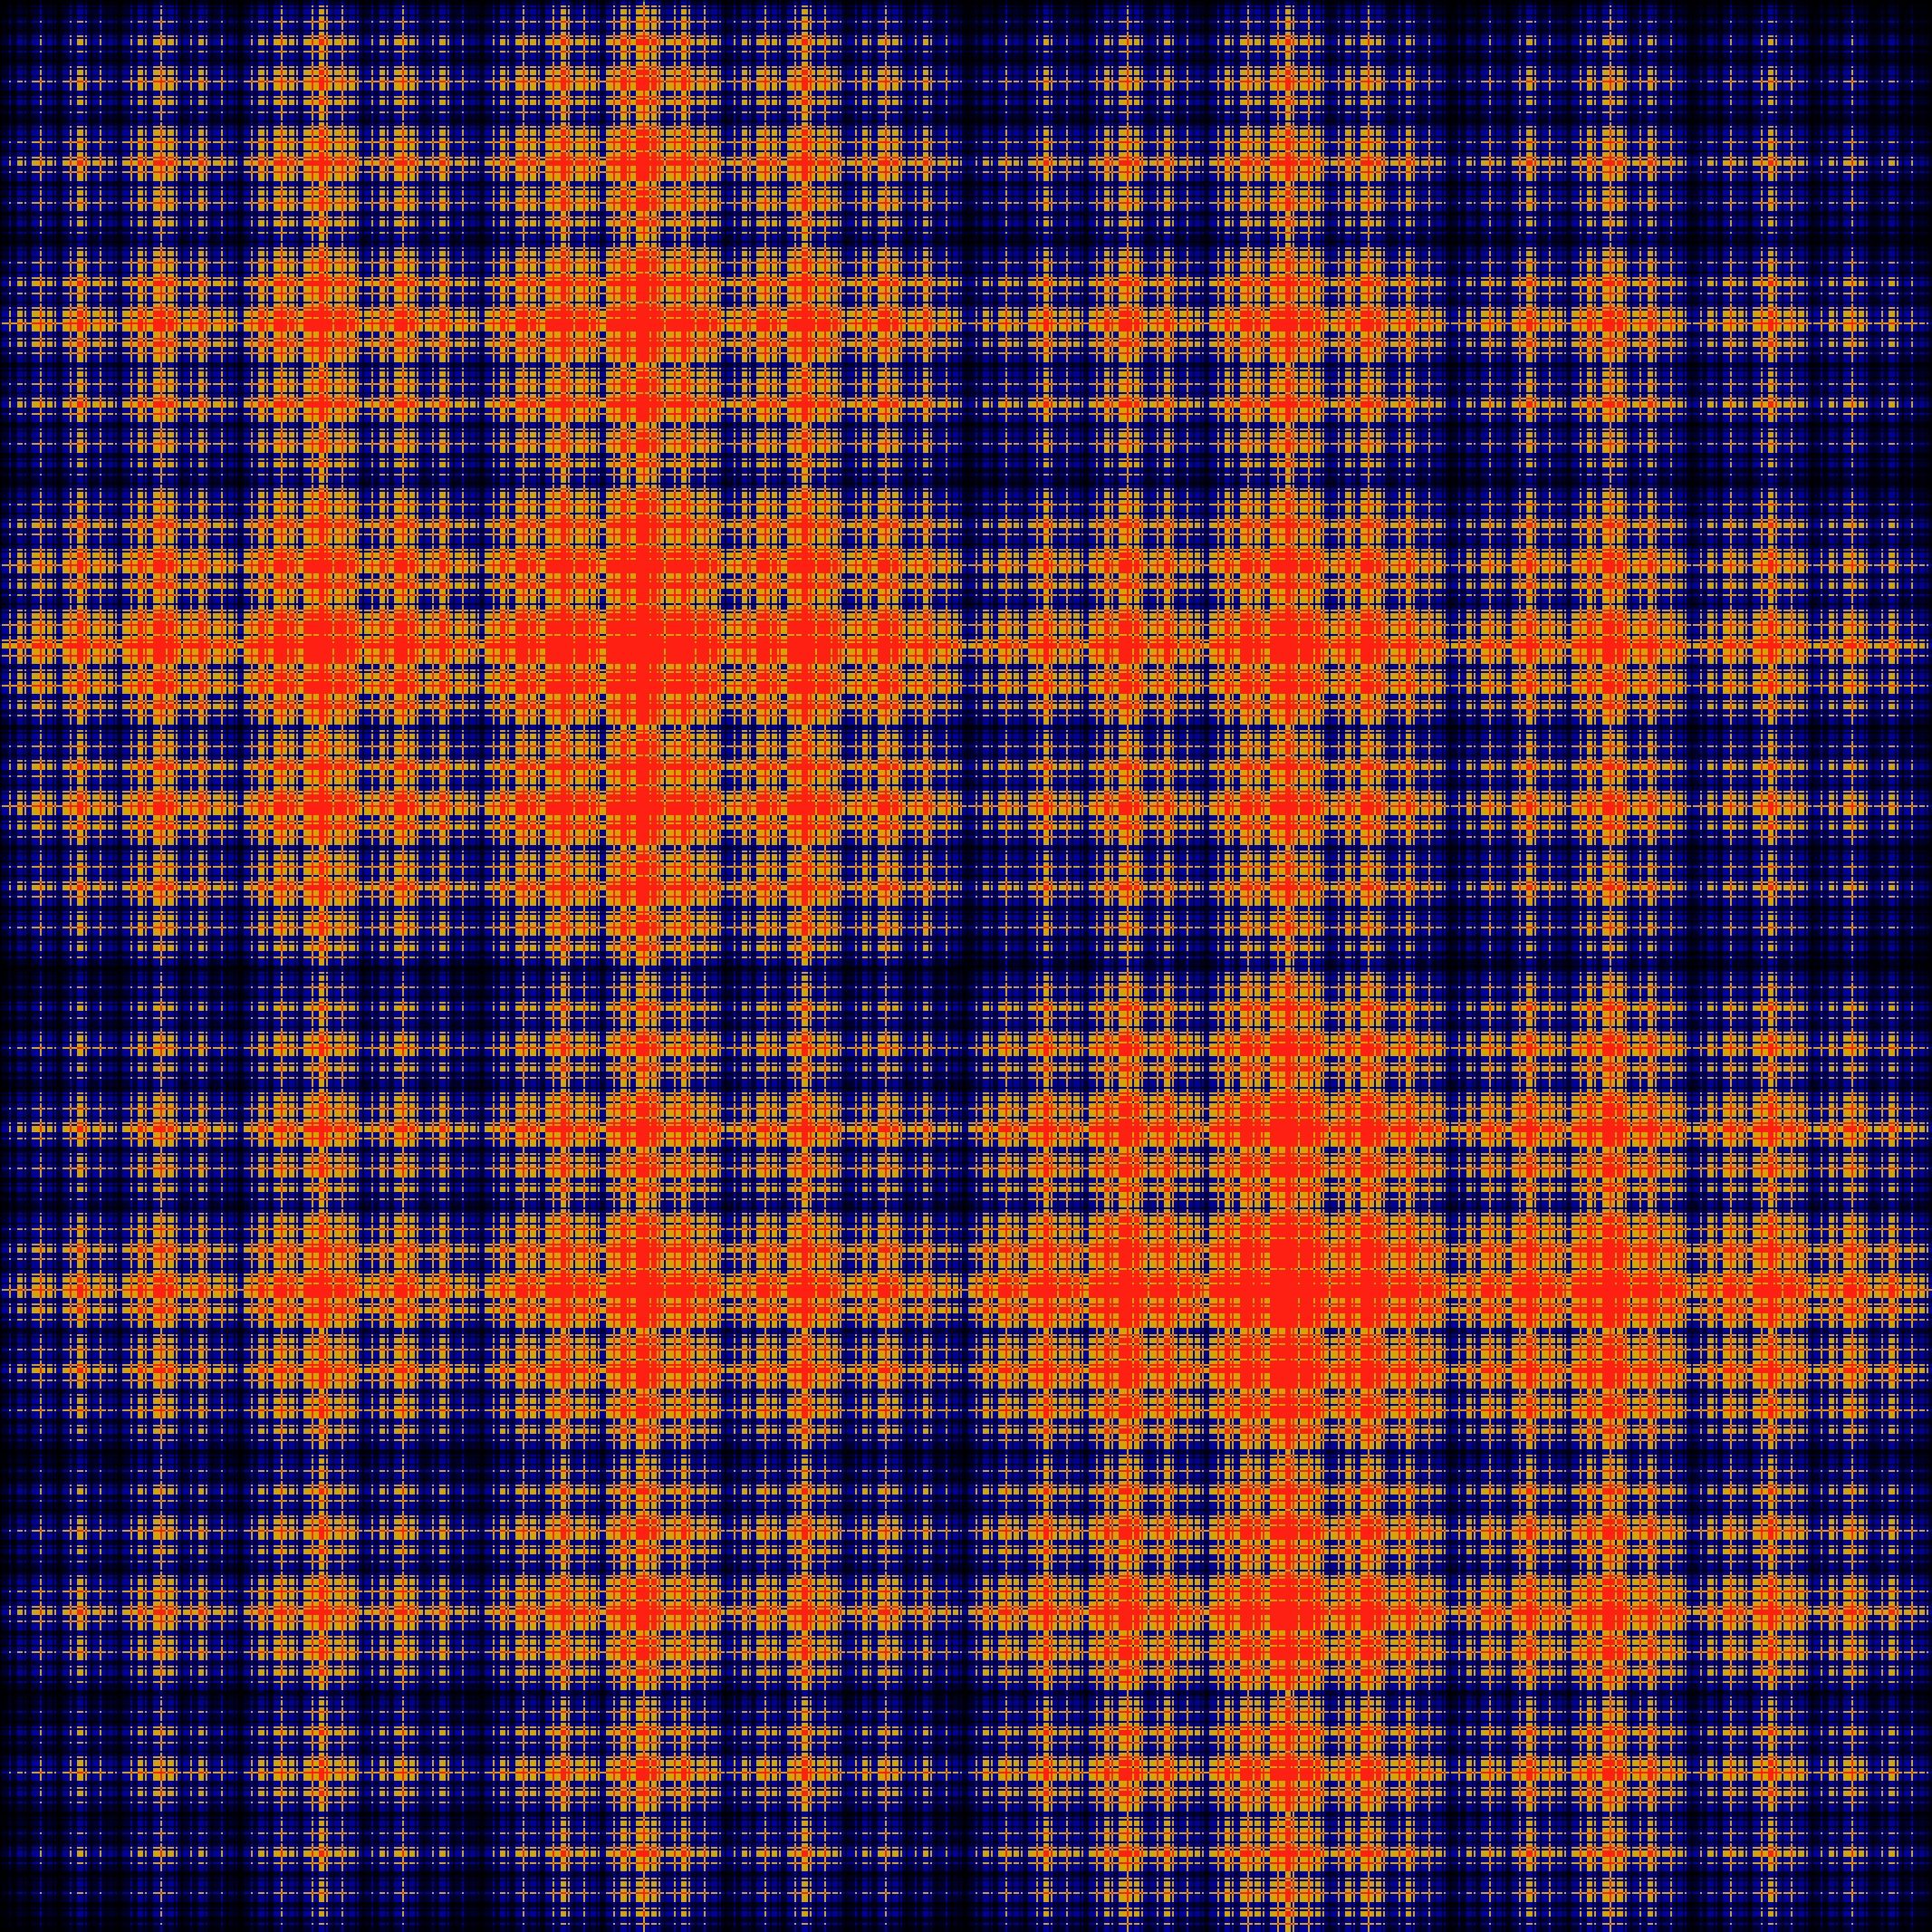
\includegraphics[scale = .25]{Cover}
\end{center}
\frontmatter
\begin{contributors}
\contributor{J.~Humpherys}{Brigham Young University}
\contributor{J.~Webb}{Brigham Young University}
\contributor{R.~Murray}{Brigham Young University}
\contributor{J.~West}{University of Michigan}
\contributor{R.~Grout}{Brigham Young University}
\contributor{K.~Finlinson}{Brigham Young University}
\contributor{A.~Zaitzeff}{Brigham Young University}
\end{contributors}

%------------------------------------------------------------------
%The preface, which will presumably be longer in the future

\begin{thepreface}
This lab manual is designed to accompany the textbook \emph{Foundations of Applied Mathematics} by Humpherys and Jarvis.

\vfill
\copyright{This work is licensed under the Creative Commons Attribution 3.0 United States 
License.  You may copy, distribute, and display this copyrighted work only if you give 
credit to Dr.~J.~Humpherys. All derivative works must include an attribution to Dr.~J.~Humpherys as the owner of this work as well as the web address to 
\\\centerline{\url{https://github.com/byuimpact/numerical_computing}}\\ as the original source of 
this 
work.\\To view a copy of the Creative Commons Attribution 3.0 License, 
visit\\\centerline{\url{http://creativecommons.org/licenses/by/3.0/us/}} or send a letter to 
Creative Commons, 171 Second Street, Suite 300, San Francisco, California, 94105, USA.}

\vfill
\centering
\includegraphics[height=1.2cm]{by}
\vfill
\end{thepreface}
%-----------------------------------------------------------------

\setcounter{tocdepth}{1}
\tableofcontents

\mainmatter

\part{Measure Theory}

\part{Random Spaces and Variables}

\part{Distributions}

\part{Limit Theorems}

\part{Markov Processes}

\part{Poisson Distributions, Queues, and Renewal}

\part{Martingales and Diffusion}

\part{Information Theory}

\part{Multivariable Statistics}
\subimport{./Algorithms/PCA/}{PCA}

\part{State Estimation}
\subimport{./Algorithms/HMMStates/}{hmmstates}

\part{Time Series}

\part{Expectation Maximization}
\subimport{./Algorithms/HMMTrain/}{hmmtrain}

\part{Bayesian Statistics I}
\subimport{./Algorithms/BayesianUpdate/}{bayesianupdate}

\part{Bayesian Statistics II}
\subimport{./Algorithms/Metropolis/}{metropolis}
\subimport{./Applications/IsingModel/}{isingmodel}

\part{Machine Learning I}



\subimport{./Applications/CrimeMapping/}{crimemapping}

\part{Machine Learning II}
\subimport{./Algorithms/KNNSVM/}{knnsvm}

\end{document}
